\chapter{Design und Designentscheidungen}
%Modul Überblick-bild
Die Betriebssoftware wurde in Module aufgeteilt, wobei eine Code-Datei einem
Modul zugeordnet ist und ein Module mehrere Code-Dateien umfassen kann.
Es wurde besonderer Wert darauf gelegt, dass Module so wenig wie möglich andere
Module aufrufen und dies auch nur durch Funktionen und nicht durch Variablen.
Dieses Prinzip musste allerdings während der Optimierungs- und Testphase
geringfügig aufgeweicht werden, da entweder der Code dadurch unleserlich wurde
oder der Preis für einen Funktionsaufruf zu hoch war in Relation zu dem
Nutzen, der dadurch erzielt wurde.
Somit gibt es nun vier bis fünf globale Variablen, die sich während der Laufzeit
ändern können und in unterschiedlichen Modulen direkt referenziert werden.
Geändert werden diese allerdings nur in sehr wenigen Funktionen, in denen dies
auch explizit Kommentiert wurde. Außerdem wurde in den Coding-Guidelines extra
auf den Umstand hingewiesen wenn möglich keine Funktionen zu schreiben, die die
globalen Variablen verändern und wenn doch dies explizit zu dokumentieren.
Neben diesen maximal fünf Verhaltensverändernden globalen Variablen gibt es vier
weitere Variablen in zwei verschiedenen Modulen, die jeweils aus einem anderen
Modul explizit gesetzt werden. Dies sind die Trigger-Werte für die Position und
die Zeit. Diese werden nur durch den Drive, bzw den Advanced Drive Befehl
gesetzt und während der Motor Interrupts nach und nach dekrementiert.
Über die Module wird in den Unterkapiteln genauer eingegangen.
\section{System}
Das als System bezeichnete Modul beinhaltet die Hauptschleife der Betriebssoftware,
sowie die Initialisierung aller anderen Submodule. Es benutzt ein paar wenige Module
um seine Aufgabe in einem abstrakten Maße zu erfüllen. Während der Hauptschleife, die
in gekürzter Fassung (Kommentare und Debug-Ausgaben entfernt) in Abb. \ref{main_loop} zu sehen,
werden nur ein paar wenige Funktionen aufgerufen, die die wichtigen Module auf dem
aktuellen Stand halten und damit es ermöglichen, dass Daten zwischen den Modulen
fließen kann.
\begin{figure}[htb]
 \centering
 \scalebox{0.5}{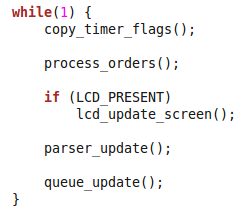
\includegraphics{pictures/main_loop_code.png}}
 \caption{\label{main_loop}Die Hauptschleife}
\end{figure}
\section{Debug}
Eigene Mechanismen zum Debugging sind genau dann sehr wichtig, wenn man nicht mit den
gewohnten Werkzeugen dies tun kann. Während der Laufzeit verstehen was in dem kleinen
Microcontroller vor sich geht ist essentiel, allerdings auch nicht sehr simpel, denn
die einzigen Möglichkeiten, die die Platine hat mit der Aussenwelt zu kommunizieren
beschränken sich auf 5 LED's, ein 4*20 Zeichen LCD, eine USART und eine I2C-Bus 
Schnittstelle. Der Aussagegehalt von den LED's (insbesondere da diese sich geweigert
haben zuverlässig zu funktionieren) und der LCD ist doch sehr begrenzt (man kann nicht
viele Informationen auf einem 4*20 Zeichen LCD unterbringen). Die Wahl fiel dann auf
die USART Schnittstelle, da der Arbeitscomputer, an dem das Debugging durchgeführt wurde
einen solchen Anschluss besitzt, aber über keinen I2C Anschluss verfügt.
Mithilfe der Debugausgaben kann man protokollieren, was das System in jedem
Schleifendurchlauf getan hat und dadurch das Verhalten analysieren, um schlussendlich
Fehler aufzuspüren. 
\section{Drive, Motor und PID}
Das Motor bindet zum einen das System an die Motoren und an die anderen nötigen
Fahrelemente an, wohingegen das Drive Modul die Services, die das Motor Modul anbietet
abstrahiert und in einer weise Zusammenfasst, die es dem System erlaubt auf sehr einfache
Art und Weise die Motoren zu bedienen.
Das PID Modul, welches größtenteils aus der vorhergegangen Studienarbeit übernommen wurde
\cite{STUD_TIMO}, ist für den Fehlerausgleich der Radbewegungen zuständig. Genauer: Es
errechnet die korrigierten Werte für die Räder, die dann vom Drive Modul an diese auch
weiter geleitet werden. Die Fehler die auftreten können sind vielfältig und nicht besonders
groß, wie zum Beispiel eine kleine Varianz in der Geschwindigkeit eines Rades oder ähnliches.
Damit aber das Fahrverhalten stabiler wird müssen diese Fehler korrigiert werden.
\section{IO, I2C und USART}
Das IO Modul stellt für das System einheitliche Funktionen zur Verfügung um Daten zu lesen als
auch zu schreiben. Hierbei kann es dem Benutzer der Funktionen egal sein, welche Schnittstelle
letztendlich für die Kommunikation genutzt wird. Das IO Modul kümmert sich um die Unterschiede
zwischen USART und I2C.
Sowohl das I2C als auch das USART Modul kümmern sich hauptsächlich um das Initialisieren der
Hardware und das behandeln der Interrupt Service Routinen.
\section{Order und Queue}
Das Order Modul ist das größte aller Module. Es beinhaltet zum einen den Typ, mit dem Befehle
intern dargestellt und verarbeitet werden. Aufbauend auf den Typ, dem einige unterstützende
Funktionen zugeteilt sind um wiederkehrende Aufgaben zu erleichtern, existiert im Order
Modul auch die Order Funktionen. Diese Order Funktionen sind Handler-Funktionen für die
im Protokoll spezifizierten Befehle. Falls ein Befehl länger benötigt, bis er als beendet
gelten kann, wird die entsprechende Order Funktion mit dem korrespondierenden Befehl in jeder
Iteration der Hauptschleife aufgerufen. Diese kann dann eventuell Wartungsarbeiten an dem
Befehl durchführen und überprüfen, ob dieser beendet ist und entsprechend seinen Status ändern.
Durch diesen Aufbau ist eine Hauptschleifeniteration sehr kurz, aber auch komplizierte Befehle
oder solche deren Parameter und Durchführung überwacht werden müssen sind hierdurch möglich.\\
Durch das Queue Modul ist es möglich der Motorplatine mehrere Befehle direkt hintereinander
zu übermitteln, die dann einer nach dem anderen ausgeführt werden, außerdem kümmert die
Queue sich darum, das Prioritäts-Befehle nicht eingereiht werden sondern bei der nächsten
Hauptschleifeniteration ausgeführt werden.
\section{Timer, Parser und Options}
Diese drei Module haben hauptsächlich eine unterstützende Funktion, so bringt das Timer Modul
die Möglichkeit mit in bestimmten zeitlichen Intervallen Befehle auszuführen. Der Parser
fasst einzelne Bytes logisch zu Befehlen zusammen und übergibt diese der Queue. Das Options
Modul beinhaltet die Einstellungen, die das Verhalten des gesamten Systems beeinflussen, wie
z.B. ob Debugging Ausgaben aktiviert sind, mit was für einer Geschwindigkeit das ABS bremst
und einiges mehr.
